\section{Specifica dei test}
\label{specificatest}
Il gruppo ha deciso di utilizzare il modello a V, come modello di sviluppo del software per assicurare la \glo{qualità} del prodotto. Questo modello illustra le relazioni tra ogni \glo{fase} del ciclo di vita di sviluppo e la fase di test ad essa associata.
\subsection{Test di sistema}
Lo scopo dei test di sistema è quello di verificare che i requisiti espressi nel documento \AdRv{4.0} vengano rispettati. Di seguito l'elenco di questi test con la loro descrizione.
\begin{longtable}{|c| C{10cm} |C{3cm}|}
	\rowcolor{darkblue}
	\textcolor{white}{\textbf{ID Test}}&
	\textcolor{white}{\textbf{Descrizione}}&
	\textcolor{white}{\textbf{Implementato}}\label{tab:TestSistema1}\\
	TRFO1 & Viene verificato che l'utente non autenticato possa registrarsi ed eseguire l'accesso  con e-mail e password come acquirente & Implementato\\ \hline
	TRFO2 & Viene verificato che l'utente non autenticato con credenziali venditore possa eseguire l'accesso alla piattaforma & Implementato\\ \hline
	TRFO3 & Viene verificato che l'utente non autenticato in possesso di credenziali acquirente possa eseguire l'accesso alla piattaforma & Implementato \\ \hline
	TRFO4 & Viene verificato che l'utente in possesso di credenziali possa modificare la password dimenticata & Implementato\\ \hline
	TRFO5 & Viene verificato che l'utente non autenticato possa accedere alla schermata di login da qualsiasi schermata della piattaforma & Implementato\\ \hline
	TRFO6 & Viene verificato che l'utente autenticato possa eseguire il logout dalla piattaforma & Implementato\\ \hline
	TRFO7 & Viene verificato che l'utente non autenticato o l'acquirente possa cercare i prodotti dalla schermata principale o dalla PLP & Implementato\\ \hline
	TRFO8 & Viene verificato che l'utente non autenticato o l'acquirente possa filtrare i prodotti della PLP per categoria, prezzo e disponibilità in magazzino & Implementato\\ \hline
	TRFO9 & Viene verificato che l'utente non autenticato o l'acquirente visualizzi i prodotti della PLP ordinati alfabeticamente come ordinamento predefinito & Implementato\\ \hline
	TRFO10 & Viene verificato che l'utente non autenticato o l'acquirente possa visualizzare nella PLP una lista di tutti i prodotti corrispondenti alla ricerca con le relative informazioni di:nome, prima immagine, prezzo e se disponibile in magazzino & Implementato \\ \hline
	TRFO11 & Viene implementato che i prodotti nella PLP non disponibili devono essere distinti da quelli che lo sono & Implementato \\ \hline
	TRFO12 & Viene verificato che l'utente non autenticato o l'acquirente possa ordinare i prodotti risultanti dalla ricerca appena effettuata per ordine alfabetico, prezzo crescente e decrescente & Implementato \\ \hline
	TRFO13 & Viene verificato che l'utente non autenticato o l'acquirente possa aggiungere al carrello i prodotti direttamente dalla PLP & Implementato\\ \hline
	TRFO14 & Viene implementato che l'utente non autenticato o l'acquirente possa accedere alla PDP di un prodotto in evidenza dalla schermata principale, riepilogo ordine e PLP & Implementato \\ \hline
	TRFO15 & Viene verificato che l'utente non autenticato o l'acquirente possa visualizzare dalla PDP:nome del prodotto, descrizione, categorie alle quali appartiene, foto, prezzo e sconti & Implementato \\ \hline
	TRFO16 & Viene verificato che l'utente non autenticato o l'acquirente possa aggiungere un prodotto al carrello direttamente dalla PDP  & Implementato\\ \hline
	TRFO17 & Viene verificato che l'utente non autenticato o l'acquirente possa modificare la quantità del prodotto che vuole aggiungere nel carrello & Implementato\\ \hline
	TRFO18 & Viene verificato che l'utente non autenticato o l'acquirente possa accedere al carrello da qualsiasi schermata della piattaforma & Implementato \\ \hline
     TRFO19 & Viene verificato che l'utente non autenticato o l'acquirente possa visualizzare il proprio carrello con il prezzo totale e l'elenco dei prodotti con le relative informazioni & Implementato\\ \hline
   	TRFO20 & Viene verificato che l'utente non autenticato o l'acquirente possa eliminare un prodotto o modificarne la quantità dal proprio carrello & Implementato\\ \hline
	TRFO21 & Viene verificato che l'utente non autenticato possa aggiungere prodotti al carrello come ospite e, appena si autentica, vengano aggiunti al suo carrello personale & Implementato\\ \hline
	TRFO22 & Viene verificato che il carrello dell'acquirente venga salvato in remoto e sia accessibile da qualsiasi dispositivo & Implementato\\ \hline
   	TRFO23 & Viene verificato che l'acquirente possa procedere all'acquisto del carrello & Implementato\\ \hline
   	TRFO24 & Viene verificato che l'acquirente possa aggiungere un nuovo indirizzo di consegna & Implementato\\ \hline
   	TRFO25 & Viene verificato che l'acquirente possa modificare l'indirizzo di consegna durante l'operazione di checkout & Implementato\\ \hline
	TRFO26 & Viene verificato che l'acquirente possa eliminare un indirizzo di consegna precedentemente inserito & Implementato\\ \hline
	TRFO27 & Viene verificato che l'acquirente possa accedere alla schermata con tutti gli ordini effettuati da qualsiasi schermata della piattaforma & Implementato \\ \hline
	TRFO28 & Viene verificato che l'acquirente possa visualizzare l'elenco degli ordini effettuati sulla piattaforma & Implementato\\ \hline
	TRFO29 & Viene verificato che l'acquirente possa visualizzare l'elenco dei prodotti acquistati in un determinato ordine, visualizzando per ognuno di essi: nome, quantità, prezzo totale & Implementato\\ \hline
	TRFO30 & Viene verificato che l'acquirente possa cercare un ordine utilizzando il suo codice & Implementato\\ \hline
	TRFO31 & Viene verificato che l'acquirente possa filtrare temporalmente gli ordini effettuati sulla piattaforma & Implementato\\ \hline
	TRFO32 & Viene verificato che l'acquirente possa accedere alla schermata con le proprie informazioni da qualsiasi altra schermata della piattaforma & Implementato\\ \hline
	TRFO33 & Viene verificato che l'acquirente, nella propria schermata principale, possa visualizzare le proprie informazioni personali, quali:nome, cognome ed indirizzo e-mail collegato & Implementato\\ \hline
	TRFO34 & Viene verificato che l'acquirente possa modificare le proprie informazioni personali:nome, cognome, e-mail e password & Implementato\\ \hline
	TRFO35 & Viene verificato che l'acquirente possa eliminare il proprio account & Implementato\\ \hline
	TRFO36 & Viene verificato che l'utente non autenticato o l'acquirente, nella schermata principale, possa visualizzare i prodotti in evidenza e la descrizione dell'azienda & Implementato\\ \hline
	TRFO37 & Viene verificato che l'utente non autenticato o l'acquirente possa accedere alla schermata principale da qualsiasi altra schermata della piattaforma & Implementato\\ \hline
    TRFO38 & Viene verificato che il venditore possa modificare le proprie informazioni personali:nome, cognome, e-mail, password, descrizione azienda & Implementato\\ \hline
	TRFO39 & Viene verificato che il venditore possa accedere alla schermata con le proprie informazioni da qualsiasi altra schermata della piattaforma & Implementato\\ \hline
    TRFO40 & Viene verificato che il venditore, nella propria schermata personale, possa visualizzare:nome, cognome, e-mail, logo, descrizione e nome dell'azienda & Implementato\\ \hline
	TRFO41 & Viene verificato che il venditore possa accedere alla propria PLP da qualsiasi schermata & Implementato\\ \hline
	TRFO42 & Viene verificato che il venditore possa visualizzare i prodotti nella PLP ordinati alfabeticamente come ordinamento predefinito & Implementato\\ \hline
	TRFO43 & Viene verificato che il venditore possa visualizzare una lista di tutti i prodotti corrispondenti alla ricerca, dove per ognuno sarà visualizzabile:nome, prima immagine, prezzo e disponibilità o meno in magazzino & Implementato\\ \hline
	TRFO44 & Viene verificato che il venditore possa accedere alla PDP di un prodotto acquistato dalla schermata di riepilogo ordine & Implementato\\ \hline
	TRFO45 & Viene verificato che il venditore possa accedere alla PDP di un prodotto dalla propria PLP & Implementato\\ \hline
    	TRFO46 & Viene verificato che il venditore possa aggiungere un nuovo prodotto alla piattaforma & Implementato\\ \hline
    	TRFO47 & Viene verificato che il venditore possa visualizzare il nome, la descrizione, le categorie, il prezzo, lo sconto, le foto e la quantità disponibile dei suoi prodotti & Implementato\\ \hline
    	TRFO48 & Viene verificato che il venditore possa modificare le informazioni di un prodotto precedentemente inserito nella piattaforma & Implementato\\ \hline
    	TRFO49 & Viene verificato che il venditore possa aggiungere un prodotto alla sezione dei prodotti in evidenza presente nella schermata principale & Implementato\\ \hline
    	TRFO50 & Viene verificato che il venditore possa rimuovere un prodotto dalla sezione dei prodotti in evidenza  presente nella schermata principale & Implementato\\ \hline
    	TRFO51 & Viene verificato che il venditore possa eliminare un prodotto precedentemente inserito nella piattaforma & Implementato\\ \hline
    	TRFO52 & Viene verificato che il venditore possa rifornire un prodotto precedentemente inserito che sta per esaurirsi o è esaurito, dalla PDP del prodotto o dalla PLP & Implementato\\ \hline
   	TRFO53 & Viene verificato che il venditore possa cercare i prodotti dalla propria PLP attraverso delle parole & Implementato\\ \hline
    	TRFO54 & Viene verificato che il venditore possa filtrare i prodotti della PLP per categoria, prezzo, disponibilità in magazzino e se è in evidenza o meno & Implementato\\ \hline
	TRFO55 & Viene verificato che il venditore possa accedere alla pagina di gestione delle categorie da qualsiasi schermata & Implementato\\ \hline
    	TRFO56 & Viene verificato che il venditore possa aggiungere una nuova categoria & Implementato\\ \hline
    	TRFO57 & Viene verificato che il venditore possa modificare una categoria precedentemente inserita & Implementato\\ \hline
   	TRFO58 & Viene verificato che il venditore possa eliminare una categoria precedentemente inserita & Implementato\\ \hline
    	TRFO59 & Viene verificato che il venditore possa cercare una categoria dalla propria schermata di amministrazione delle categorie & Implementato\\ \hline
	TRFO60 & Viene verificato che il venditore possa visualizzare il nome di tutte le categorie attualmente inserite nella piattaforma & Implementato\\ \hline
	TRFO61 & Viene verificato che il venditore possa visualizzare gli ordini chiusi o da gestire & Implementato\\ \hline
    	TRFO62 & Viene verificato che il venditore, nella schermata riepilogo ordini,  possa visualizzare una lista dei prodotti acquistati in un determinato ordine & Implementato\\ \hline
    	TRFO63 & Viene verificato che il venditore possa modificare lo stato di un determinato ordine & Implementato\\ \hline
	TRFO64 & Viene verificato che il venditore possa visualizzare gli ordini ricevuti per ordine cronologico decrescente come ordinamento predefinito & Implementato\\ \hline
	TRFO65 & Viene verificato che il venditore possa cercare un ordine dalla propria schermata di riepilogo ordini per codice e cliente & Implementato\\ \hline
    	TRFO66 & Viene verificato che il venditore possa filtrare gli ordini per lo stato dell'ordine secondo un intervallo temporale ordinandoli in base alla data di accettazione & Implementato\\ \hline
	\rowcolor{white}
    	\caption{Descrizione dei test di sistema.}
\end{longtable}
\begin{longtable}{|c| C{13cm}|}
	\rowcolor{white}
	\rowcolor{darkblue}
	\textcolor{white}{\textbf{ID Test}}&
	\textcolor{white}{\textbf{ID Requisito}}\label{tab:TestSistema2}\\
	TRFO1 & RFO1\_1, RFO2\_1.1.1, RFO3\_1.1.2, RFO4\_1.1.3, RFO5\_1.1.4, RFO6\_1.1.5\\ \hline
	TRFO2 & RFO7\_2\\ \hline
	TRFO3 & RFO7\_2\\ \hline
	TRFO4 & RFO8\_3\\ \hline
	TRFO5 & RFO9\\ \hline
	TRFO6 & RFO10\_4\\ \hline
	TRFO7 & RFO11\_5\\ \hline
	TRFO8 & RFO12\_6, RFO13\_6.1, RFO14\_6.2, RFO15\_6.3\\ \hline
	TRFO9 & RFO16\\ \hline
	TRFO10 & RFO17\\ \hline
	TRFO11 & RFO18\\ \hline
	TRFO12 & RFO19\_7, RFO20\_8, RFO21\_9\\ \hline
	TRFO13 & RFO22\_10\\ \hline
	TRFO14 & RFO23, RFO24, RFO25, RFO26\\ \hline
	TRFO15 & RFO27\\ \hline
	TRFO16 & RFO28\_11\\ \hline
	TRFO17 & RFO29\_12\\ \hline
	TRFO18 & RFO30\\ \hline
	TRFO19 & RFO31\_13, RFO32\_13\\ \hline
	TRFO20 & RFO33\_14, RFO33\_15\\ \hline
	TRFO21 & RFO35\\ \hline
	TRFO22 & RFO36\\ \hline
	TRFO23 & RFO37\_16, RFO38, RFO39, RFO40\_16.1\\ \hline
	TRFO24 & RFO41\_17, RFO42\_17.1.1, RFO43\_17.1.2, RFO44\_17.1.3, RFO45\_17.1.4\\ \hline
	TRFO25 & RFO46\_18, RFO47\_18.1, RFO48\_18.2, RFO49\_18.3, RFO50\_18.4\\ \hline
	TRFO26 & RFO51\_19\\ \hline
	TRFO27 & RFO52\\ \hline
	TRFO28 & RFO53\_20\\ \hline
	TRFO29 & RFO54\_20\\ \hline
	TRFO30 & RFO55\_21\\ \hline
	TRFO31 & RFO56\_22, RFO57\_22.1, RFO58\_22.2\\ \hline
	TRFO32 & RFO59\\ \hline
	TRFO33 & RFO60\\ \hline
	TRFO34 & RFO61\_23, RFO62\_23.1, RFO63\_23.2, RFO64\_23.3\\ \hline
	TRFO35 & RFO65\_24\\ \hline
	TRFO36 & RFO66\\ \hline
	TRFO37 & RFO67\\ \hline
	TRFO38 & RFO68\_25, RFO69\_25.1, RFO70\_25.2, RFO71\_25.3, RFO72\_26\\ \hline
	TRFO39 & RFO73\\ \hline
	TRFO40 & RFO74\\ \hline
	TRFO41 & RFO75\\ \hline
	TRFO42 & RFO76\\ \hline
	TRFO43 & RFO77\\ \hline
	TRFO44 & RFO78\\ \hline
	TRFO45 & RFO79\\ \hline
	TRFO46 & RFO80\_27, RFO81\_27.1, RFO82\_27.2, RFO83\_27.3, RFO84\_27.4, RFO85\_27.5, RFO86\_27.6, RFO87\_27.7\\ \hline
	TRFO47 & RFO88\\ \hline
	TRFO48 & RFO89\_28, RFO90\_28.1, RFO91\_28.2, RFO92\_28.3. RFO93\_28.4, RFO94\_28.5, RFO95\_28.6, RFO96\_28.7\\ \hline
	TRFO49 & RFO97\_29\\ \hline
	TRFO50 & RFO98\_30\\ \hline
	TRFO51 & RFO99\_31\\ \hline
	TRFO52 & RFO100\_32\\ \hline
	TRFO53 & RFO101\_33\\ \hline
	TRFO54 & RFO102\_34, RFO103\_34.1, RFO104\_34.2, RFO105\_34.3, RFO106\_34.4\\ \hline
	TRFO55 & RFO107\\ \hline
	TRFO56 & RFO108\_35, RFO109\_35.1\\ \hline
	TRFO57 & RFO110\_36, RFO111\_36.1\\ \hline
	TRFO58 & RFO112\_37\\ \hline
	TRFO59 & RFO113\_38\\ \hline
	TRFO60 & RFO114\\ \hline
	TRFO61 & RFO115\_39\\ \hline
	TRFO62 & RFO116\_39\\ \hline
	TRFO63 & RFO117\_40\\ \hline
	TRFO64 & RFO118\\ \hline
	TRFO65 & RFO119\_41, RFO120\_42\\ \hline
	TRFO66 & RFO121\_43, RFO122\_43.1, RFO123\_43.2, RFO124\_43.2.1, RFO125\_43.2.2\\ \hline
	\rowcolor{white}
	\caption{Relazione tra test di sistema e requisiti.}\\
\end{longtable}
\newpage
\subsection{Test di unità}
Lo scopo dei test di unità è quello di isolare ciascuna parte di un programma e mostrarne correttezza e completezza nell'\glo{implementazione}, facendo emergere eventuali difetti, in modo che essi possano essere corretti prima dell'integrazione. I test d'unità sono stati effettuati attraverso l'utilizzo di \glo{Jest.js}, la valutazione sull'andamento degli stessi è stata effettuata considerando il valore medio del code coverage. Di seguito si riporta il grafico relativo all'andamento del code coverage medio durante il periodo di progettazione di dettaglio.
\begin{figure}[ht]
	\centering
	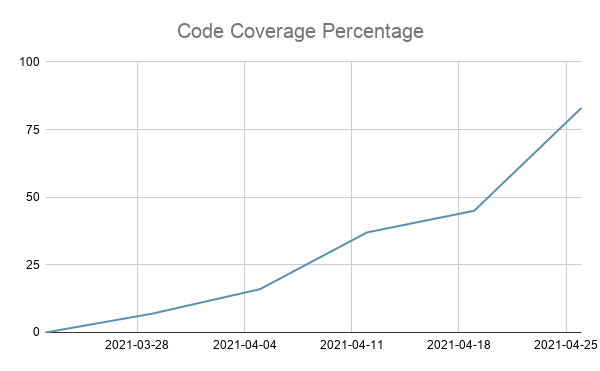
\includegraphics[scale=0.5]{Immagini/TestUnit}\\
	\caption{Code coverage test unità}
	\label{fig:CodeCoverage}
\end{figure}
\subsection{Test di integrazione}
Lo scopo dei test di integrazione è quello di verificare che l'unione di più parti di codice porti al risultato atteso. Per i test d'integrazione è stato utilizzata la funzionalità messa a disposizione del glo{framework} Serverless, la misura di riferimento è il numero di chiamate \glo{REST}.
\begin{figure}[ht]
	\centering
	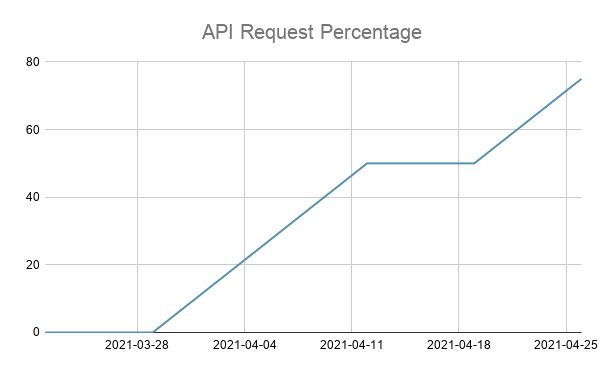
\includegraphics[scale=0.5]{Immagini/TestInteg}\\
	\caption{Percentuale chiamate API REST}
	\label{fig:ChiamateREST}
\end{figure}
